\documentclass[a4paper]{article}

\usepackage{polski}
\usepackage[utf8]{inputenc}
\usepackage[pdftex]{graphicx}
\usepackage{fancyhdr}
\usepackage{float}

\newcommand{\prog}{\texttt}

\linespread{1.15}
\pagestyle{fancy}
\fancyhf{}
\chead{Sprawozdanie końcowe}
\cfoot{Strona \thepage \ z \pageref{end}}

\title{Sprawozdanie końcowe \\ Projekt \textit{Gra Galaxy Defender} w języku Java}
\author{Jakub Czajka (299239) \\ Daniel Daczko (299241)}

\begin{document}
\maketitle
\tableofcontents
\thispagestyle{empty}
\newpage

\section{Wprowadzenie teoretyczne}
Naszym zadaniem było stworzenie gry typu \textit{multiplayer shooter}. Nasz program nazwaliśmy \textit{Galaxy Defender}. Wykorzystuje ona grafikę dwuwymiarową. Gra inspirowana jest dwoma klasycznymi tytułami:
\begin{itemize}
    \item \textit{Space Invaders}, z których czerpie sposób eliminacji wrogów, poruszanie się gracza oraz zbieranie punktów,
    \item \textit{Tetris}, z których czerpie kształt wrogów oraz ich sposób poruszania się.
\end{itemize}
Rozgrywka rozpoczyna się od pojawienia się na ekranie dwóch statków przypisanych do graczy. Gracze mogą poruszać się horyzontalnie i ustawiać kąt działka laserowego.
Nie mogą oni jednak zamienić się miejscami (tzn. gracz, który zaczął grę po lewej stronie nie może przejść na prawo za gracza, który rozpoczął grę po prawej i na odwrót).
Wraz z~upływem czasu pojawia się pierwsza fala wrogów.\\ \\
Zadaniem graczy jest zestrzelenie klocków w jak najkrótszym czasie. Za każde zbicie użytkownik otrzymuje punkty.
Wraz z każdą kolejną minutą gry gra ulega utrudnieniu. Klocki zmniejszają się, zaczynają poruszać się szybciej i~tworzyć bardziej złożone formy.\\ \\
Jeżeli wróg dotrze do linii statków, zostają odjęte punkty od wyników obydwu graczy. Gra kończy się automatycznie, kiedy jeden z wyników wskaże liczbę ujemną. 
Dodatkowo gracze w dowolnej chwili mogą zakończyć grę i zapisać jej wynik w celu późniejszej kontynuacji.
\\
\begin{figure}[H]
    \centering
    
\includegraphics[]{img/ikona.png}
    \caption{Ikona programu}
    \label{fig:ikona}
\end{figure}

\section{Jakie założenia wstępne udało się spełnić?}
Udało nam się zaimplementować w programie wszystkie przewidywane funkcjonalności, jest to:
\begin{enumerate}
    \item Możliwość rozpoczęcia nowej gry.
    \item Wczytywanie z plików domyślnej konfiguracji programu.
    \item Możliwość wczytania gry z pliku tekstowego o własnym rozszerzeniu \textit{Galaxy Defender Game (*.gdg)}.
    \item Możliwość wprowadzania imion graczy.
    \item Możlwiość sterowania statkami kosmicznymi.
    \item Wyświetlanie na bieżąco zdobytych przez graczy punktów.
    \item Wyświetlanie czasu gry.
    \item Możliwość zatrzymania gry.
    \item Możliwość wznowienia gry.
    \item Możliwość zapisania aktualnego stanu gry do pliku tekstowego w rozszerzeniu programu \textit{Galaxy Defender Game (*.gdg)}.
    \item Obsługa błędów powstałych na skutek wczytania niepoprawnej zawartości pliku tekstowego lub problemem z dostępem do niego.
    \item Obsługa błędów powstałych na skutek wprowadzania niepoprawnych ciągów znaków w pole \textit{imię gracza}.
    \item Możliwość wyświetlenia instrukcji do gry.
    \item Zaprogramowanie utrudnienia gry postępującego w czasie.
\end{enumerate}

\section{Jakich zadań nie udało się zrealizować?}
Niestety nie wszystkie założenia i cele zostały przez nas w pełni zrealizowane. Jest to przede wszystkim:
\begin{enumerate}
    \item Zachowanie systematyczności zamieszczania testów programu w repozytorium.
    \item Uniknięcie zmian podczas kodowania w stosunku do specyfikacji implementacyjnej.
    \item Przetestowanie działania programu w systemie operacyjnym MacOS X.
    \item Dodanie animacji podczas niszczenia klocków.
    \item Dodanie animacji podczas poruszania statkami.
    \item Usytuowanie miejsca startowego laserów pod statkami.
    \item Unormowanie prędkości laserów.
    \item Dopracowanie graficznego przedstawienia kolizji statków.
    \item Dodanie efektów dźwiękowych do programu.
    \item Dodanie możliwości zatrzymania gry klawiszem ESC.
\end{enumerate}

\section{Przykładowe uruchomienia}
Poniższe ilustracje przedstawiają przykładowe ekrany działania programu:
\begin{figure}[H]
    \centering
    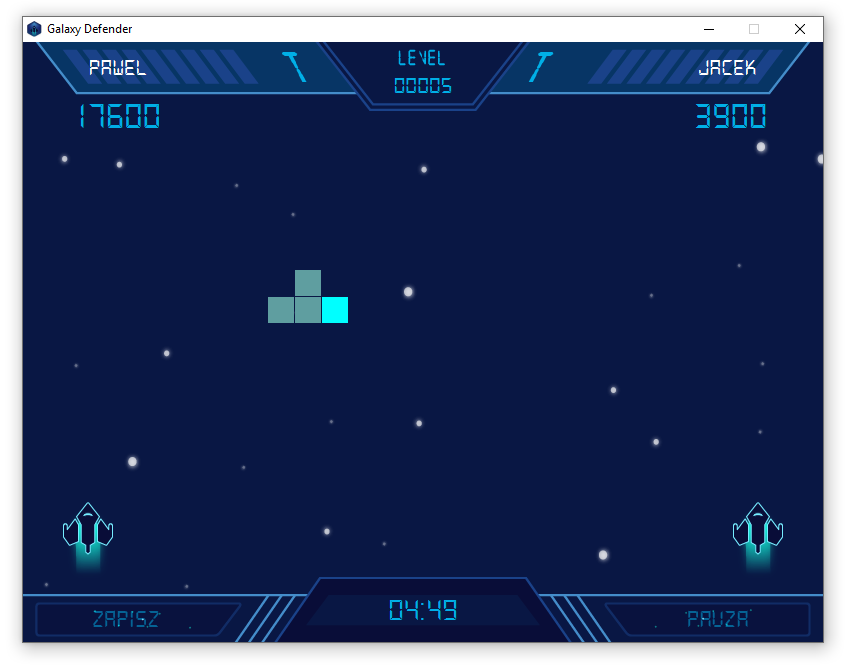
\includegraphics[width=1\textwidth]{img/ekran-gry-screenshot.png}
    \caption{Ekran gry}
    \label{fig:game}
\end{figure}

\begin{figure}[H]
    \centering
    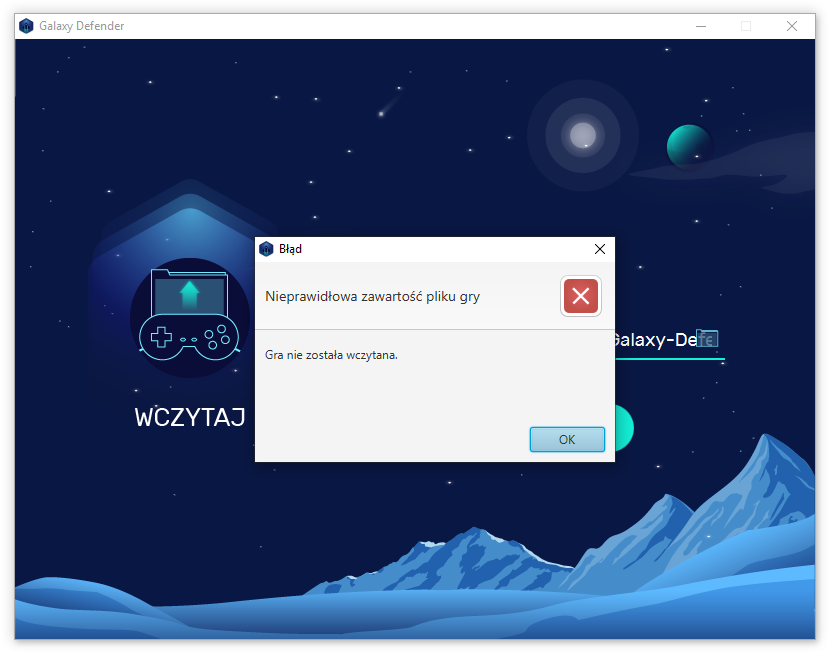
\includegraphics[width=1\textwidth]{img/ekran-wczytywania-screenshot.png}
    \caption{Ekran wczytywania i alert błędu}
    \label{fig:read}
\end{figure}

\begin{figure}[H]
    \centering
    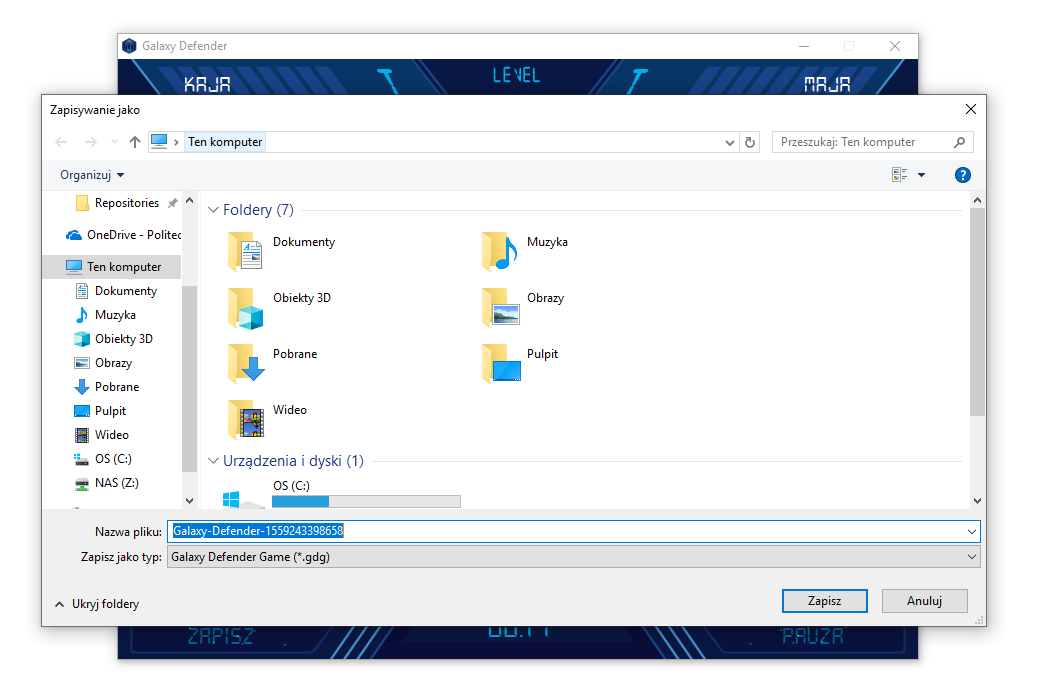
\includegraphics[width=1\textwidth]{img/zapisywanie-gry-screenshot.png}
    \caption{Okno dialogowe zapisu gry}
    \label{fig:save}
\end{figure}

\section{Rozbieżności względem specyfikacji}
\subsection{Specyfikacja funkcjonalna}
Delikatnym modyfikacjom uległa \textbf{struktra katalogów}, która obecnie wygląda w~następujący sposób:
\begin{figure}[H]
    \centering
    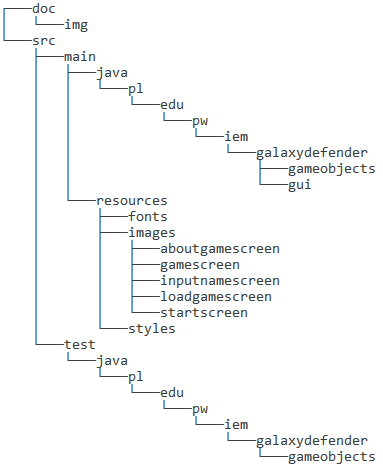
\includegraphics[width=0.5\textwidth]{img/struktura-katalogow.png}
    \caption{Struktura katalogów w projekcie}
    \label{fig:cat}
\end{figure}

\subsection{Specyfikacja implementacyjna}
\begin{enumerate}
    \item Rozszerzenie klas o dodatkowe metody oraz pola, tak aby kod był napisany w sposób jak najbardziej optymalny i uniwersalny.
    \item Zmiana planowanych metod w klasach spowodowana nieznajomością mechanizmów Javy.
    \item Zmiana w klasie \prog{AnimationThread}:
    \begin{enumerate}
        \item zmiana nazwy na \prog{GameAnimation}, aby klasa nabrała nazwy znaczącej,
        \item rozszerzanie klasy \prog{AnimationTimer} spowodowane poznaniem plusów podanej klasy. W odróżnieniu do Threada, klasa ta działa dokładnie raz na klatkę wykonaną w scenie, co przynosi wiele korzyści przy rozpatrywaniu trafienia klocka.
    \end{enumerate}
    \item Zmiana układu budowy GUI.
    \item Wykorzystanie klasy Button do utworzenia przycisków spowodowane zapoznaniem się z mechanizmem plików .css współpracujących z JavaFX.
    \item Wykorzystanie biblioteki JUnit.
    \item Zmiana konwencji pisania testów. Klasy testujące mają nazwy klas, które testują z dopiskiem Test.
\end{enumerate}

\section{Mechanizmy Java 1.8 zastosowane w projekcie}
Jedynym mechanizmem pochodzącym z Javy w wersji 1.8 jest metoda \prog{sizeToScene} klasy Stage (\prog{javafx.stage}). Ustawia ona szerokość i wysokość obiektu klasy \prog{Window}, aby dopasować rozmiar zawartości tej sceny do okna.

\section{Aktualna wersja diagramu klas}
Ze względu na rozmiar diagramu klas rozbiliśmy go na trzy diagramy dla poszczególnych pakietów:
\begin{figure}[H]
    \centering
    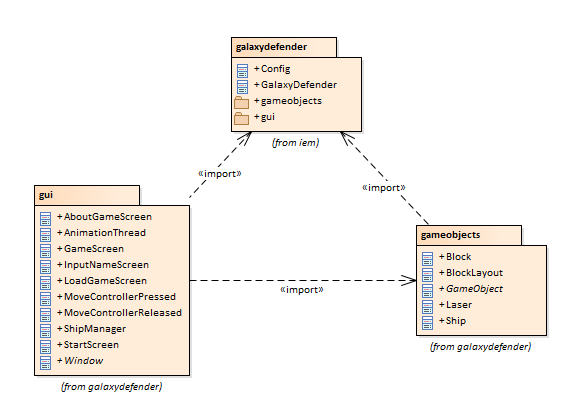
\includegraphics[width=1\textwidth]{img/packages.png}
    \caption{Diagram pakietów}
    \label{fig:packages}
\end{figure}

\begin{figure}[H]
    \centering
    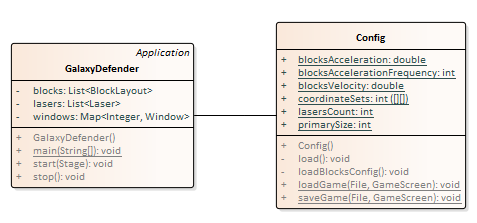
\includegraphics[width=0.75\textwidth]{img/pakiet-galaxydefender.png}
    \caption{Diagram klas w pakiecie główny \textit{galaxydefender}}
    \label{fig:pack1}
\end{figure}

\begin{figure}[H]
    \centering
    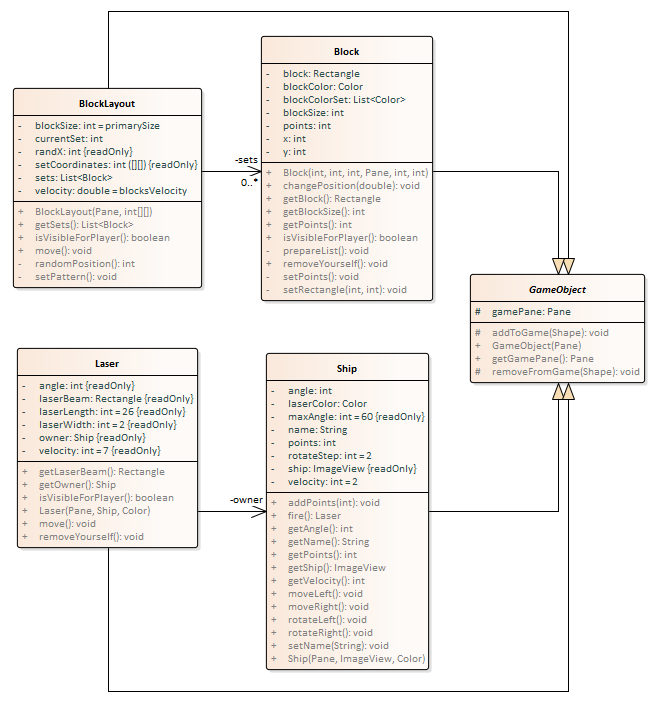
\includegraphics[width=1\textwidth]{img/pakiet-gameobjects.png}
    \caption{Diagram klas w pakiecie \textit{galaxydefender.gameobjects}}
    \label{fig:pack1}
\end{figure}

\begin{figure}[H]
    \centering
    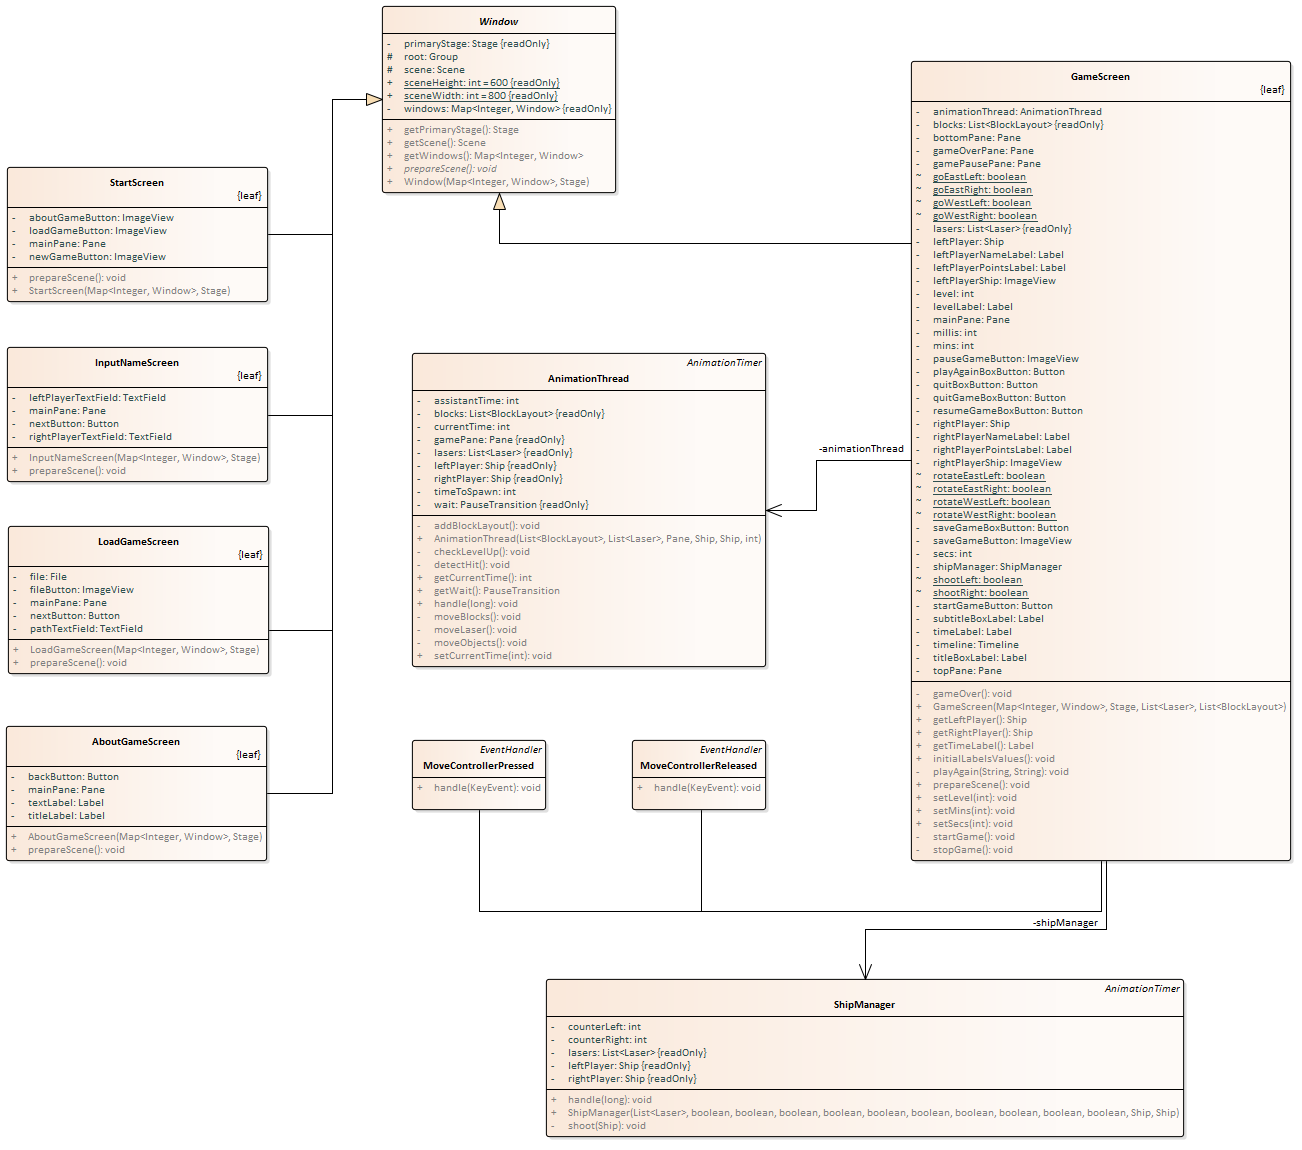
\includegraphics[width=1\textwidth]{img/pakiet-gui.png}
    \caption{Diaram klas w pakiecie \textit{galaxydefender.gui}}
    \label{fig:pack1}
\end{figure}

\section{Testy programu}
\paragraph{}Funkcjonalność poszczególnych elementów programu sprawdzaliśmy na bieżąco podczas implementacji.
Jeżeli dany komponent działał zgodnie z założeniami, dołączaliśmy go do programu.
W tym celu pomocne okazało się wykorzystanie testów białej skrzynki.
Dodatkowo dla klas obiektów gry napisaliśmy testy jednostkowe.
\paragraph{}Główne testy nastąpiły po zaimplementowaniu podstawowych mechanik rozgrywki.
W tym momencie nasze testy polegały na przeprowadzeniu rozgrywki i~sprawdzaniu zachowań programu podczas różnych okoliczności.
\paragraph{}Ostatecznie program oddaliśmy w ręce znajomych, których subiektywna ocena oraz uwagi pozwoliły nam na naprawienie i ulepszenie działania gry.
Wszystkie testy można znaleźć w katalogu \prog{src/test/java} w naszym repozytorium.

\section{Podsumowanie i wnioski}
\paragraph{}Otrzymane zadanie od początku staraliśmy się wykonać z należytym zaangażowaniem i precyzyjnością. Czyniliśmy wszelakie zabiegi, aby spełnić wszystkie postawione nam wymagania wobec działania programu. Po dokładnej analizie doszliśmy do wniosku, że udało nam się sprostać zadaniu. Program działa poprawnie i jest przenośny. Został on przez nas rozszerzony w rozmaitych detalach.
\paragraph{}Największą trudność sprawiło nam napisanie specyfikacji i przewidzenie struktury kodu, czego przyczyną mogła być krótka znajomość programowania w języku Java. Niestety nie udało nam się uniknąć zmian w stosunku do wcześniej przygotowanych dokumentów.
\paragraph{}Nasza współpraca przebiegała pomyślnie. Dopełnialiśmy się na każdym etapie wykonywania projektu. Pozytywnie oceniamy systematyczność naszej pracy i~atmosferę wspólnego działania.
\paragraph{}Programowanie zdecydowanie ułatwiło nam korzystanie z rozproszonego systemu kontroli wersji Git i zintegrowanego środowiska programistycznego NetBeans. Bardzo przydatnym narzędziem automatyzującym budowę oprogramowania okazał się Apache Maven.
\paragraph{}W trakcie realizacji zadania zrozumieliśmy kwintesencję pisania specyfikacji przed rozpoczęciem samego programowania, co na pewno przyczyni się do bardziej profesjonalnego rozwiązywania kolejnych problemów programistycznych, które staną na naszej drodze podczas studiów i później w pracy zawodowej.
\label{end}

\end{document}